\section{Instrumentation} \label{sec:myoband}
	% former Myo armband -section
%What does the band consist of?
%Electrodes, gyroscope and accelerometer
%Build-in filters and stuff like that?
%Sampling frequency

%head
The following section will contain a presentation of the Myo armband from Thalmic Labs, which will be used for data acquisition in this study and an explanation of acquiring EMG signals using surface electrodes.

\subsection{Myo armband}

The Myo armband is a device developed by Thalmic Labs capable of identifying hand gestures and arm movements in order to interact and control different electronic devices. The system can be used with software provided by Thalmic Labs to control a limited range of devices using the data from the armband.
%However, standard use of the system does not provide use of the raw data, which is necessary for this project. The system does however allow data to be extracted from the armband, with without involving the software from Thalmic Labs. This enables to acquire data to process in Matlab. 
The Myo armband is illustrated in \figref{fig:armband}. 

\begin{figure}[H]                    
	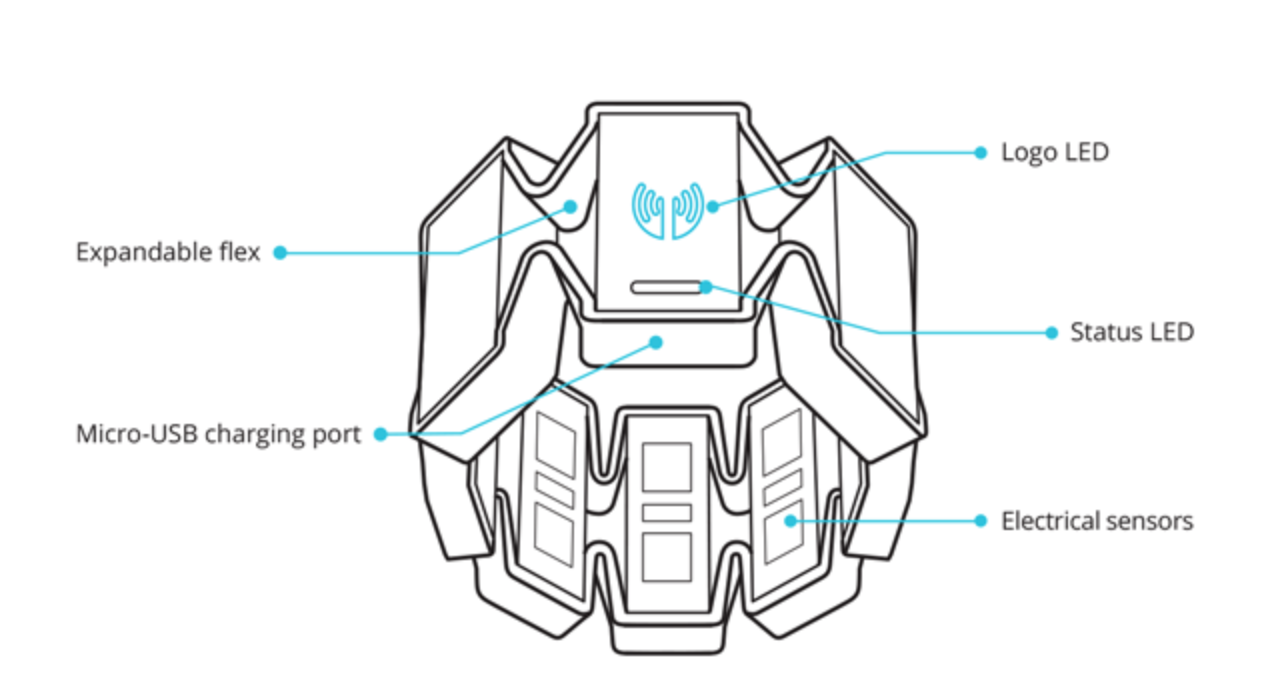
\includegraphics[width=.5\textwidth]{figures/myob/armband}  %<--but is not needed.
	\caption{Main components of the Myo armband. \textbf{SOURCE}}
	\label{fig:armband}  %<--give the figure a label, so you can reference!
\end{figure}


%The main components of the Myo armband illustrated in the figure \ref{fig:armband} are:
%\begin{itemize}
%\item The logo LED gives information about the sync state. The LED is solid when you perform the Sync Gesture successfully and
%the Myo armband is synced to your arm. The LED pulses when the armband is not synced.
%\item The status LED shows the state of the Myo armband. When it lights up in blue once the Myo armband is connected to a device. 
%\item The USB charging port allows to charge the Myo armband battery. 
%\end{itemize}
%The systems counts with sizing clips, these small pieces give a tighter grip which is more appropriated for smaller arms.

The Myo armband has eight medical grade stainless steel surface EMG sensors. %responsible of recognizing each gesture. 
These electrodes are dry and therefore not covered in silver chloride gel to reduce impedance between the electrode and skin. However, it has been shown by Mendez et al. \cite{Mendez2017} that the EMG recorded with the Myo armband is a suitable acquisition system for mapping hand gestures compared to conventional EMG acquisition. The only mapping method used in that study was linear discriminant analysis, and it is noted that other mapping methods should be investigated to further validate the quality of mapping the EMG obtained by the Myo armband. The Myo armband is sampling sEMG data at a sample rate of 200 Hz. A low sample rate could result in problems of aliasing later on in the data processing, since the range of the sEMG signal is 10-500 Hz. \cite{cram2012} 

In addition, it has a nine axis inertial measurement unit (IMU) which enable the detection of arm movement. An IMU is an electronic device that provides information concerning position and orientation for navigation and stabilization purposes. The IMU's in the Myo armband comprises a three axis accelerometer, a three axis gyroscope and a three axis magnetometer. The accelerometer measures the physical acceleration experienced by an object, where the object in this case is the body part where the Myo armband is placed. 
%It gives information about the acceleration experienced relative to free fall and expresses this in g-force. One g-force being when the accelerometer is at rest on the Earth's surface. That is since all points on the surface of the Earth is accelerating upwards relative to an object in free fall near the surface. For the g-force to change from one g-force the accelerometer must be exposed to motion. 
The gyroscope has the property of measuring angluar velocity. The magnetometer has the property of a compass, measuring the earth's magnetic field. This enables the armband to provide data on orientation. IMU data is sampled at a sample rate of 50 Hz. The Myo armband communicates through Bluetooth 4.0 to a computer.
%(something about the actual data the myoband provides and how many axes a magnometer actually has). \textbf{SOURCE}
%\textbf{more text on the data types we are going to get from the IMU's} 
% ... (It is equipped with an ARM Cortex-M4 microprocessor of low energy consumption.)

%\begin{figure}[H]                    
%	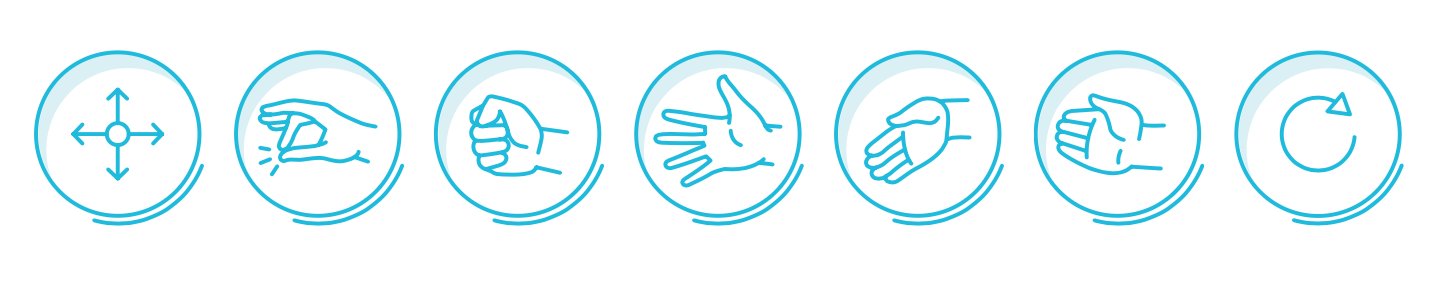
\includegraphics[width=.5\textwidth]{figures/myob/gestures}  %<--but is not needed.
%	\caption{Hand gestures and movements detected by the Myo armband using its own interface from Thalmic Labs. SOURCE}
%	\label{fig:gestures}  %<--give the figure a label, so you can reference!
%\end{figure}
%It offers five pre-defined gestures as showed in the figure \ref{fig:gestures}, it provides haptic feedback through short, medium or long vibrations to correct moves or activate the system.

%JACOVB COMENT:sample rate high enough


%This means that many high-frequencies of the sEMG signal will not be recorded, and aliasing could have an influence on the recorded signals due to not respecting the Nyquist Law of sample rate. 
%Thus, the Myo band arm supplies two kinds of data, the IMU data and EMG data. %which is spatial and gestural. 
%The IMU data add information about the orientation and movement of the user's arm. This information is provided through the accelerometer and the gyroscope. EMG recordings gives information about the users hand gestures. The recorded signals can be send to other devices using Bluetooth 4.0.


%/begin{figure}
%poner imagen del los gestos%
%/end{figure}

%How does it communicate with the computer?
%Connection
%Programs that can be used to interface with the arm
%What kind of data will be received from the myo band?


%it connecrs to a PC or tablet via bluetooth Low Energy and allows both raw data streaming and the use of a proprietary library for gesture recognition.The signal processing is performed on the host platform and the used algorithms are not documented (poner de otra manera)


